% 2. Methods
%   2.1. Chaste
%   2.2. Morphometric model
%     2.2.1. CT image processing: lung segmentation, centerline and radii extraction
%     2.2.2. Generation of the statistical part
%   2.3. Julia Programming Language
%     2.3.1. «ModelingToolkit.jl» handles model complexity
%     2.3.2. Callbacks role in state variables discontinuity handling
%   2.4. Mechanical model
%     2.4.1. Blocks description
%     2.4.2. Model testing on a subtree

% 2. Methods
\section{Methods}
% Visione d'insieme (diagramma con flusso dell'informazione, data
% pipeline). Questo diagramma mostra a partire dagli input che ho
% avuto (TC) tutto l'iter del dato.

% Qui ha detto poi Chiara che conviene inserire delle informazioni
% riguardanti i modelli matematici utilizzati.

\Cref{fig:data_pipeline} provides a high-level overview of the main
operations performed.  Each of the two classes of methods correspondss
to one of the two models:

\begin{enumerate}
\item \emph{Chaste} library is utilized in the generation of
  \emph{morphometric model}.
\item \emph{Julia Programming Language} is employed to describe and
  instantiate the \emph{mechanical model}, as well as to perform
  \emph{simulations}.
\end{enumerate}

% todo: modificare l'immagine sopra ad "anatomical surrogate generation" con uno screen di ParaView.
% todo: aggiungere immagini sopra al branch del modello meccanico.

\begin{figure}[H]\centering
  \begin{tikzpicture}[node distance=3cm]
    % Nodes
    %% Chaste & Morphometric Model
    \node (ct_acquisition)           [startstop] {CT\\Acquisition};
    \node (img_ct_acquisition)       [image, above of=ct_acquisition, yshift=-1.0cm]                   {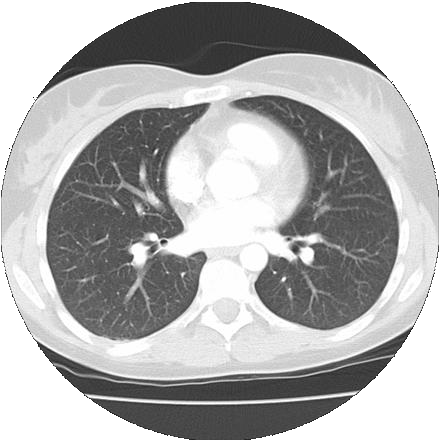
\includegraphics[width=2.0cm]{ct_acquisition.png}};
    %%% Upper branch
    \node (lobes_segmentation)       [process, right of=ct_acquisition, xshift=3.25cm, yshift=+2cm]    {Lobes\\segmentation};
    %%% Lower branch
    \node (img_lobes_segmentation)   [image, above of=lobes_segmentation, xshift=-.1cm, yshift=-1.2cm] {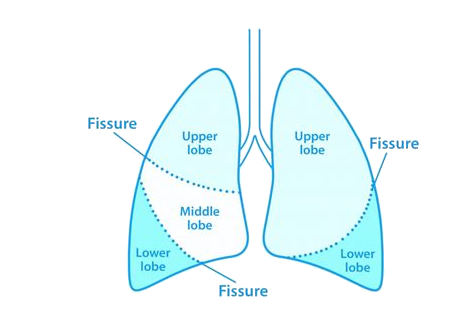
\includegraphics[width=3.5cm]{lobes_segmentation.png}};
    \node (airways_segmentation)     [process, below of=lobes_segmentation, xshift=-2cm, yshift=-1cm]  {Airways\\segmentation};
    \node (img_airways_segmentation) [image, above of=airways_segmentation, xshift=2cm, yshift=-1cm]   {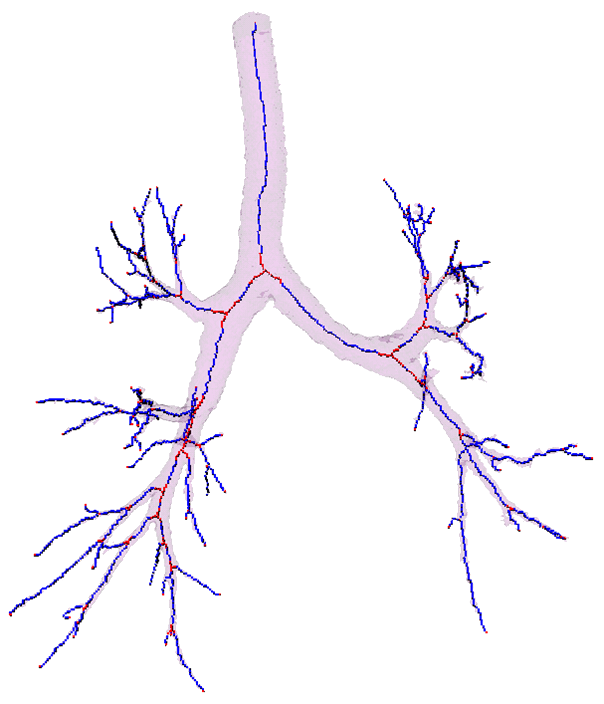
\includegraphics[height=2.5cm]{airways_segmentation.png}};
    \node (centerline_extraction)    [process, below of=lobes_segmentation, xshift=+2cm, yshift=-1cm]  {Centerline\\extraction};
    \node (surrogate_generation)     [process, right of=ct_acquisition, xshift=9.5cm]                  {Anatomical surrogate\\generation};
    \node (img_surrogate_generation) [image, above of=surrogate_generation, yshift=-.5cm]              {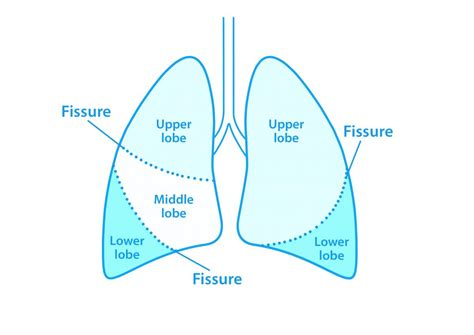
\includegraphics[width=3.5cm]{lobes_segmentation.jpg}};
    %% Julia & Mechanical Model
    \node (parameters_update)        [process, below of=ct_acquisition, yshift=-3cm]                   {Lungs parameters\\update};
    \node (model_instantiation)      [process, right of=parameters_update, xshift=1cm]                 {Mechanical model\\instantiation};
    \node (DAE_solution)             [process, right of=model_instantiation, xshift=1cm]               {DAE System\\solution};
    \node (simulations)              [startstop, right of=DAE_solution, xshift=+1cm]                   {Mechanical Simulations};

    % Arrows
    \draw [arrow] (ct_acquisition.east)                              -- ++(.5,0) coordinate(tmp)     |- (airways_segmentation.west);
    \draw [arrow] (airways_segmentation)                             -- (centerline_extraction);
    \draw [arrow] (centerline_extraction.east)                       -- ++(.5,0) coordinate(tmp1)    |- (surrogate_generation.west);
    \draw [arrow] (model_instantiation)                              -- (DAE_solution);
    \draw [arrow] (DAE_solution)                                     -- (simulations);
    \draw [arrow] (tmp)                                              |-   (lobes_segmentation.west);
    \draw [arrow] (lobes_segmentation)                               --   (tmp1|-lobes_segmentation) |- (surrogate_generation.west);
    \draw [dashed, thick, ->,>=stealth] (surrogate_generation.south) -- ++(0,-3.5)                   -| (parameters_update.north);
    \draw [arrow] (parameters_update)                                -- (model_instantiation);

    % Frame around a part of the flowchart
    \begin{pgfonlayer}{background}
      \node[rounded corners=3mm,
      draw=blue,
      thick, dashed,
      fit=(airways_segmentation)(centerline_extraction)(img_lobes_segmentation)(img_surrogate_generation),
      fill=cyan!5,
      inner sep=7pt,
      label={[anchor=north]below:\textsc{\textcolor{blue}{Chaste \& Morphometric model}}}] {};
    \end{pgfonlayer}
    \begin{pgfonlayer}{background}
      \node[rounded corners=3mm,
      draw=red,
      thick, dashed,
      fit=(parameters_update)(model_instantiation)(DAE_solution),
      fill=magenta!5,
      inner sep=7pt,
      label={[anchor=north]below:\textsc{\textcolor{red}{Julia Programming Language \& Mechanical model}}}] {};
    \end{pgfonlayer}
  \end{tikzpicture}
  \caption{Data pipeline.  The process begins with a
    \emph{patient-specific image} (i.e. CT) of a premature newborn.
    The extracted data, comprising \emph{two segmentations}, are then
    processed to obtain an anatomical surrogate of the airway tree.
    This is necessary due to scanner resolution not allowing for the
    discrimination and localization of small branches.  From the
    resulting morphometric model, the \emph{mechanical parameters} can
    be derived, which are essential for generating an accurate
    simulation model.  Finally, a numerical solver for differential
    equations provides the final output.}
    \label{fig:data_pipeline}
\end{figure}

%%% Local Variables:
%%% mode: LaTeX
%%% TeX-master: "../Thesis"
%%% End:


%   2.1. Chaste
\subsection{Chaste}
\label{subsec:chaste}

Chaste is a C++ open-source (BSD licensed) library developed by Oxford
University.  It has multiple use cases across various biomedical
fields, with an emphasis on cardiac electrophysiology and cancer
development\cite{mirams2013}.  It can be integrated into a C++ program
or used via «User Project» (i.e. \texttt{ctest}).
Specifically, the ``AirwayGenerationTutorial'' is considered as a
first codebase and properly adapted to match newborn
parameters\cite{airwaygeneration2024}.

The required input consists of two pieces of information:
\begin{itemize}
\item A \emph{mesh of centerline points}.  This mesh is provided in
  TetGen format, comprising ``airways.node'' and ``airways.edge''
  files. The first file lists centerline points coordinates,
  respective sampled airways radius and a boolean value to indicate if
  the point is generative. The second one contains all the connections
  between pairs of points.
\item Four (or five) \emph{lobes segmentations} in STL format.  These
  segmentations are necessary as they physically impose a limit on the
  growth algorithm.
\end{itemize}

%   2.2. Morphometric model
\subsection{Morphometric Model}
\label{subsec:morphometric_model}
% Per Chiara: Inserisco definizione di modello morfometrico?

%     2.2.1. CT, centerline and radii extraction
\subsubsection{CT Image Processing: Lung Segmentation, Centerline and
  Radii Extraction}
\label{subsubsec:ct_centerline_radii_extraction}
% todo: Devo chiedere bene a Francesca come sono stati estratti i
% raggi.

«3D Slicer» is an open-source software used for CT image processing.
Two extensions are installed:

\begin{description}
\item «\emph{Chest\_imaging\_platform}»: This extension enables
  semi-automatic segmentation of major airways from a single fiducial
  point.  It can also extract adult lobes using three fiducial points
  per lung fissure. However, in our case, the fissures are not
  visible, necessitating manual intervention.
\item «\emph{SlicerVMTK}»: This extension is used for extracting
  centerline points.
\end{description}

%     2.2.2. Generation of the statistical part
\subsubsection{Generation of the Statistical Portion}
\label{subsubsec:statistical_generation}

% Riferirsi a Tawhai2000.

The Chaste User Project reads the input files (see
\Cref{subsec:chaste}), and begins growing the anatomical surrogate
from the points labeled as «generative».  The algorithm operating
under the hood is a modified version of the one described in
\cite{tawhai2000}.  The generated output is available in various
formats:

\begin{itemize}
\item vtu: Unstructured Grid (base64 encoded) format used by VTK
  library.  It can be displayed by ParaView, an open-source viewer.
\item node and edge: TetGen format.  Such files are better suited for
  further processing.
\end{itemize}

%   2.3. Julia Programming Language
\subsection{Julia Programming Language}
\label{subsec:julia}

Julia is a free, open-source (MIT licensed), fast, scientific and
numerical computing-oriented programming language.  Its computational
efficiency is comparable to that of statically-typed languages like C
or Fortran.  Moreover, its high-level code expressivity rivals that of
languages like Python, R and MATLAB\cite{juliadocs2024}.

Two key features, inspired by the \emph{Lisp Language}, are
highlighted here.

\begin{description}
\item \emph{Metaprogramming}: Code is treated as any other Julia data
  structure, thus can be dynamically generated and manipulated at
  runtime.
\item \emph{Macros}: They help instantiate the generated code in the
  body of a program.
\end{description}

Their importance is closely tied to the concept of Domain-Specific
Languages (aka DSLs).  These dialects are composed by abstractions
that can be properly exploited to solve particular problems
(e.g. modeling complex systems, solving differential equations).

Julia REPL has a built-in package manager (i.e. «\texttt{Pkg.jl}»)
used for managing project dependencies and ensuring the
\emph{repeatability} of computational setups.  This is achieved by
saving the required package names and commits into `Project.toml' and
`Manifest.toml' files.

%     2.3.1. «ModelingToolkit.jl» handles model complexity
\subsubsection{«\texttt{ModelingToolkit.jl}» handles
  Model Complexity}
\label{subsubsec:modelingtoolkit}

This Julia package encompasses all the tools necessary for model
design.  \texttt{ModelingToolkit.jl}» is equation-driven, requiring
each system to be described by Differential-Algebraic Equations
(i.e. DAEs) for subsequent solving\cite{ma2021}. Its built-in DSL
optimizes every stage of modeling, from prototyping components to
instantiating the complete system.

An acausal paradigm can be adopted, allowing users to reason in terms
of \emph{components}\cite{mtkdocs2024}. This modularity facilitates
system extensibility compared to the causal approach, where the entire
system of Differential-Algebraic Equations must be considered and
manually simplified\cite{ma2024}.

In particular, the usage of \jlinl{@mtkmodel} macro enables
hierarchical generation of building blocks recurring in the
highest-order model (i.e. «Lungs»).  Here is how information is
structured within \jlinl{@mtkmodel} macro.

\begin{jllisting}[label=@mtkmodel, caption={\jlinl{@mtkmodel}: a macro for systems prototyping.}]
  @mtkmodel <name_of_model> begin
      @parameters begin
          # (Optional) Some constant (e.g. Resistance, Capacitance) ...
      end
      @components begin
          # (Optional) Some dependency system (e.g. Resistor, Capacitor) ...
      end
      @variables begin
          # (Optional) Internal variables ...
      end
      @equations begin
          # Differential Algebraic Equations describing the model's behavior.
      end
      @continuous_events begin
          # (Optional) Some callback function ...
      end
  end
\end{jllisting}

Replicating the behavior of electrical components using this language
is straightforward, once you are familiar with the syntax and
understand the Differential-Algebraic Equations that represent their
characteristics.  Each generated system can then be composed into more
complex ones, using the internal \jlinl{@components} macro, thereby
implementing the hierarchical structure mentioned earlier.

After describing the highest-order system, Julia compiler requires its
instantiation before any simulation can be performed.  This is
accomplished using \jlinl{@mtkbuild} macro, which minimizes the number
of equations that need to be solved.

%     2.3.2. Callbacks role in state variables discontinuity handling
\subsubsection{Callbacks' Role in State Variables Discontinuity
  Handling}
\label{subsubsec:callbacks}

Not all characteristics of electrical components can be defined solely
by DAEs.  Voltages or currents may suddently change, triggered by a
circuit event.  In such cases, \emph{continuous callback functions}
can be employed to appropriately alter the value of state variables.
These callbacks consist of two functions:
\begin{itemize}
\item \texttt{condition}: Specifies the event to be tested.
\item \texttt{affect}: Defines how the state variable(s) should be
  changed.
\end{itemize}

The component-based approach allows for the definition of callbacks
directly within the (sub)system being modeled.

% Example of usage?

%   2.4. Mechanical model
\subsection{Mechanical Model}
\label{subsec:morphometric_model}

Code modularity is directly reflected in the electrical equivalent
circuit.  Specifically, by encapsulating systems with the internal
\jlinl{@components} macro, it becomes possible to generate models of
increasing complexity.  This approach enables a clear separation
between components belonging to different hierarchical levels and
facilitate compartmentalization during the model design phase.

%     2.4.1. Blocks description
\subsubsection{Blocks Description}
\label{subsubsec:blocks_description}

% 1. È necessario indicare la notazione utilizzata nelle formule?
% 2. Su cosa devo concentrarmi nella descrizione? Devo mostrare
% codice?

The following blocks are listed in a bottom-up order (from lowest to
highest).

\begin{enumerate}
\item \textbf{Electrical components}.  The simplest blocks are derived
  from «\texttt{ModelingToolkitStandardLibrary}», while
  integral-dependent ones rely on a modified mathematical block to
  manage both current integration and its timing correctly.  Their
  behavior varies based on the neonatal pulmonary fluid interface.
  \begin{itemize}
  \item \emph{Current Integral-Dependent Inductor}:
    $L(t) = L_{a} + L_{b}\cdot \left(1 - \dfrac{\int {i
          dt}}{V_{\text{FRC}}}\right)$
  \item \emph{Current Integral-Dependent Resistor}:
    $R(t) = R_{a} + R_{b}\cdot \left(1 - \dfrac{\int {i
          dt}}{V_{\text{FRC}}}\right)$
  \item \emph{Diode}
  \item \emph{Inductor}
  \item \emph{Resistor}
  \end{itemize}
\item \textbf{Modules}.  Obtained by connecting the aforementioned
  components together into functional models representing a
  physiological structure.
  \begin{itemize}
  \item
    \emph{Alveolus}
  \item \emph{Airway}.  It has a similar behavior with respect to a
    transmission line.
  \end{itemize}
\item \textbf{Lungs}.  Highest order model as it is a combination of
  alveoli and airways.
\end{enumerate}

% Equivalent circuits for airways and alveolus.
\begin{figure}[H]\centering
  \begin{circuitikz}[]
    % Circuit
    %% Main branch

    %%% Input Node
    \draw (1.5,0)
    node[ocirc] (circuit_IN) {}
    to[short, i=$i_{\text{in}}$, -*] ++(1.5,0) coordinate(D_SW_IN)
    ;
    
    %%% Diode // Switch branch
    \draw (D_SW_IN)
    to[short] ++(0,.5)
    to[diode, v^<=$V_{\text{in,th}}$, color=bluePoli] ++(2,0) coordinate(D_SW_OUT)
    to[short, -*] (D_SW_IN-|D_SW_OUT)
    ;
    \draw (D_SW_IN)
    to[short] ++(0,-.5)
    to[switch, color=bluePoli, a_=$\left(V_{\text{in}}\geq V_{\text{in,th}}\right) \lor \left(V_{\text{in}} \text{ = } 0\right)$] ++(2,0)
    to[short] (D_SW_IN-|D_SW_OUT)
    ;

    %% Main branch
    \draw (D_SW_IN-|D_SW_OUT)
    to[short] ++(.5,0)
    to[variable resistor, color=bluePoli, l=$R_{\text{tube}} / 2$] ++(2,0)
    to[variable inductor, color=bluePoli, l=$I_{\text{tube}} / 2$] ++(2,0) coordinate (C_g_IN)
    to[short] ++(1.5,0) coordinate (SW_IN)
    to[variable resistor, color=bluePoli, l=$R_{\text{tube}} / 2$] ++(2,0)
    to[variable inductor, color=bluePoli, l=$I_{\text{tube}} / 2$] ++(2,0)
    to[short, i=$i_{\text{out}}$] ++(1,0)
    node[ocirc] (circuit_OUT) {}
    ;

    %%% C_g branch
    \draw (C_g_IN)
    to[C=$C_{\text{g}}$, *-] ++(0,-3.5)
    node[ground]{} ++(0,0)
    ;

    %%% Sw branch
    \draw (SW_IN)
    to[L=$I_{\text{sw}}$, *-] ++(0,-1.5)
    to[R=$R_{\text{sw}}$] ++(0,-1)
    to[C=$C_{\text{sw}}$] ++(0,-1)
    node[ground]{} ++(0,0)
    ;
    
    %% Open circuit (input)
    \draw (circuit_IN)
    to[open, -o, v<=$V_{\text{in}}$] ++(0, -3.5)
    node[ground] {}
    ;
    %% Open circuit (output)
    \draw (circuit_OUT)
    to[open, -o, v^<=$V_{\text{out}}$] ++(0, -3.5)
    node[ground] {}
    ;

    % Nodes
    %% IN
    \draw  (circuit_IN.west)
    node[draw, anchor=east, color=white, fill=bluePoli!50] (node_IN) {IN}
    ;
    % \draw (node_IN.east) node[ocirc, right]{}
    % ;
    %% OUT
    \draw  (circuit_OUT.east)
    node[draw, anchor=west, color=white, fill=bluePoli!50] (node_OUT) {OUT}
    ;
  \end{circuitikz}
  \caption{Airway equivalent circuit.  In blue: all current integral-dependent components.}
  \label{fig:airway}

\end{figure}

%%% Local Variables:
%%% mode: LaTeX
%%% TeX-master: "../Thesis"
%%% End:

\begin{figure}[H]\centering
  \begin{circuitikz}[scale=.9]
    % Circuit
    %% Main branch

    %%% Input Node
    \draw (1.5,0)
    node[ocirc] (circuit_IN) {}
    to[short, i=$i_{\text{in}}$, -*] ++(1.5,0) coordinate(D_SW_IN)
    ;
    
    %%% Diode // Switch branch
    \draw (D_SW_IN)
    to[short] ++(0,.5)
    to[diode, v^<=$V_{\text{in,th}}$, color=bluePoli] ++(2,0) coordinate(D_SW_OUT)
    to[short, -*] (D_SW_IN-|D_SW_OUT)
    ;
    \draw (D_SW_IN)
    to[short] ++(0,-.5)
    to[switch, color=bluePoli, a_=$\left(V_{\text{in}}\geq V_{\text{in,th}}\right) \lor \left(V_{\text{in}} \text{ = } 0\right)$] ++(2,0)
    to[short] (D_SW_IN-|D_SW_OUT)
    ;

    %% Main branch
    \draw (D_SW_IN-|D_SW_OUT)
    % to[short] ++(.5,0)
    to[variable resistor, color=bluePoli, l=$R_{\text{tube}}$] ++(2.25,0)
    to[variable inductor, color=bluePoli, l=$I_{\text{tube}}$] ++(2.25,0) coordinate (circuit_OUT)
    % to[short] ++(.5,0)
    to[L=$I_{\text{t}}$] ++(2.25,0)
    to[R=$R_{\text{t}}$] ++(1.5,0)
    to[C=$C_{\text{t}}$] ++(1.5,0) coordinate (S_IN)
    % node[ocirc] (circuit_OUT) {}
    ;

    \draw (S_IN)
    to[short] ++(0,-.5)
    to[R, l_=$R_{\text{s}}$] ++(2,0)
    to[short] ++(0,.5)
    ;
    \draw (S_IN)
    to[short, *-] ++(0,.5)
    to[C=$C_{\text{s}}$] ++(2,0)
    to[short] ++(0,-.5)
    to[short, *-] ++(.5,0)
    node[ground]{} ++(0,0)
    ;

    %%% C_g branch
    \draw (circuit_OUT) node[draw, anchor=south, color=white, fill=bluePoli!50] {OUT}
    to[C=$C_{\text{g}}$, i=$i_{\text{out}}$, v<=$V_{\text{out}}$, *-] ++(0,-3.5)
    node[ground]{} ++(0,0)
    ;

    %% Open circuit (input)
    \draw (circuit_IN)
    to[open, -o, v<=$V_{\text{in}}$] ++(0, -3.5)
    node[ground] {}
    ;
    % %% Open circuit (output)
    % \draw (circuit_OUT)
    % {[red!60] to[open, -o, v^<=$V_{\text{out}}$] ++(0, -3.5)}
    % node[ground] {}
    % ;

    % Nodes
    %% IN
    \draw  (circuit_IN.west)
    node[draw, anchor=east, color=white, fill=bluePoli!50] (node_IN) {IN}
    ;
    % \draw (node_IN.east) node[ocirc, right]{}
    % ;
    %% OUT

  \end{circuitikz}
  \caption{Alveolus equivalent circuit.  In blue: all current integral-dependent components.}
  \label{fig:alveolus}

\end{figure}


%     2.4.2. Model testing on a subtree
\subsubsection{Model Testing on A Subtree}
\label{subsubsec:model_testing_on_subtree}

Simulations are executed starting from a subnet, as the full circuit
(comprising over 50k modules) requires more memory space than
typically available on a common laptop.

\begin{figure}[H]
  \centering
  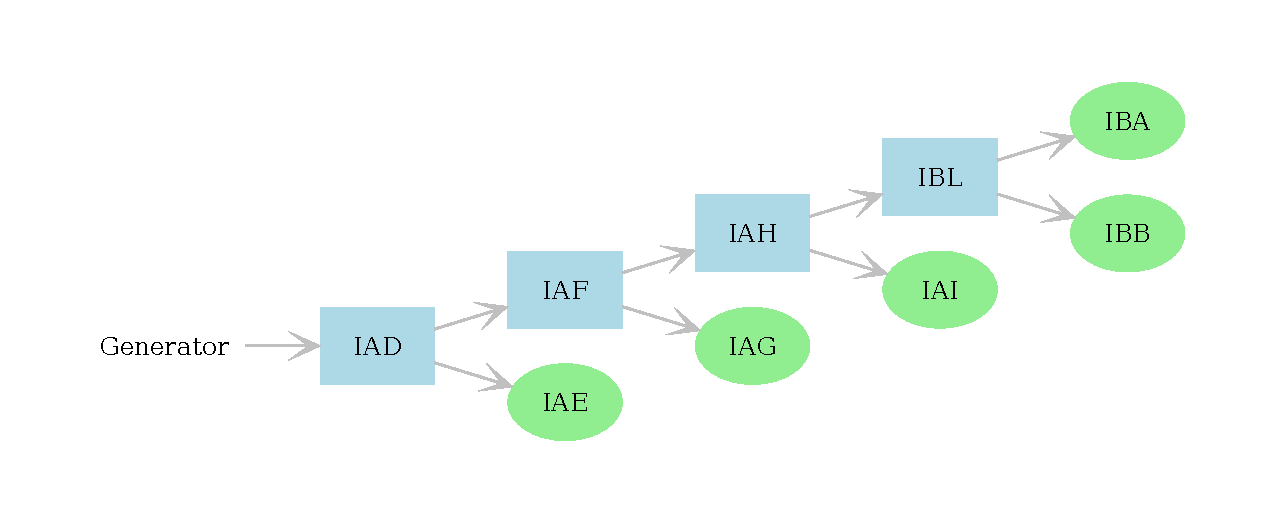
\includegraphics[scale=.7]{subtree.pdf}
  \caption{The simulated subtree.  Airways are represented in light blue, alveoli in light green.}
  \label{fig:subtree}
\end{figure}


% In this project, Chaste has been relied upon generating an anatomical
% surrogate for lungs in premature newborns.

%%% Local Variables:
%%% mode: LaTeX
%%% TeX-master: "../Thesis"
%%% End:
